\documentclass[8pt]{beamer}
\usetheme{ru}           % Use ru theme

\usepackage{common}
\usetikzlibrary{shapes.arrows}

\mode<presentation>{}

%% preamble
\title{Curve25519: Proving datatypes with a rooster}
% \subtitle{Coq }
\author[Beno\^{i}t \textsc{Viguier} MSc]{
  \normalsize Beno\^{i}t \textsc{Viguier} MSc \\
  {\small (\texttt{$\lambda$ x y. x@y.nl}) benoit viguier} \\
  {\small \url{https://www.viguier.nl}}\\ \medskip}

\institute[Radboud University Nijmegen]{
  Institute for Computing and Information Sciences -- Digital Security \\
  Radboud University Nijmegen}

\date[9, Dec. 2016]{
  DS Lunch talk \\
  9th December 2016}

\setbeamertemplate{navigation symbols}{}
\begin{document}

%%%%%%%%%%%%%%%%%%%%%%%%%%%%%%%%%
%
%			SLIDE TITLE
%
%%%%%%%%%%%%%%%%%%%%%%%%%%%%%%%%%

\begin{frame}
\titlepage
\end{frame}

%%%%%%%%%%%%%%%%%%%%%%%%%%%%%%%%%
%
%     SLIDE CONTENT
%
%%%%%%%%%%%%%%%%%%%%%%%%%%%%%%%%%

\begin{frame}{Overview}
\tableofcontents
\end{frame}

\section{A quick overview of TweetNaCl}
% \subsection{A simple language}
%%%%%%%%%%%%%%%%%%%%%%%%%%%%%%%%%
%
%			SLIDE 1
%
%%%%%%%%%%%%%%%%%%%%%%%%%%%%%%%%%
\begin{frame}[fragile]{Context}
  \begin{center}

\begin{lstlisting}[language=cnacl, caption=crypto\_scalarmult, label=cod:languageC11]
  for(i=254;i>=0;--i) {
    r=(z[i>>3]>>(i&7))&1;
    sel25519(a,b,r);
    sel25519(c,d,r);
    A(e,a,c);               #
    Z(a,a,c);               #
    A(c,b,d);               #
    Z(b,b,d);               #
    S(d,e);                 #  The steps and order
    S(f,a);                 #  of the operations
    M(a,c,a);               #  have been proved
    M(c,b,e);               #  by Timmy Weerwag
    A(e,a,c);               #
    Z(a,a,c);               #
    S(b,a);                 #  The use of datatypes
    Z(c,d,f);               #  (number representation)
    M(a,c,_121665);         #  is not proven (yet).
    A(a,a,d);               #
    M(c,c,a);               #
    M(a,d,f);               #
    M(d,b,x);               #
    S(b,e);                 #
    sel25519(a,b,r);
    sel25519(c,d,r);
  }
\end{lstlisting}

  \end{center}
\end{frame}

%%%%%%%%%%%%%%%%%%%%%%%%%%%%%%%%%
%
%     SLIDE 2
%
%%%%%%%%%%%%%%%%%%%%%%%%%%%%%%%%%
\begin{frame}[fragile]{Datatype (or number representation)}
  \begin{center}

  256 bits integers does not fit into a 64 bits containers...

  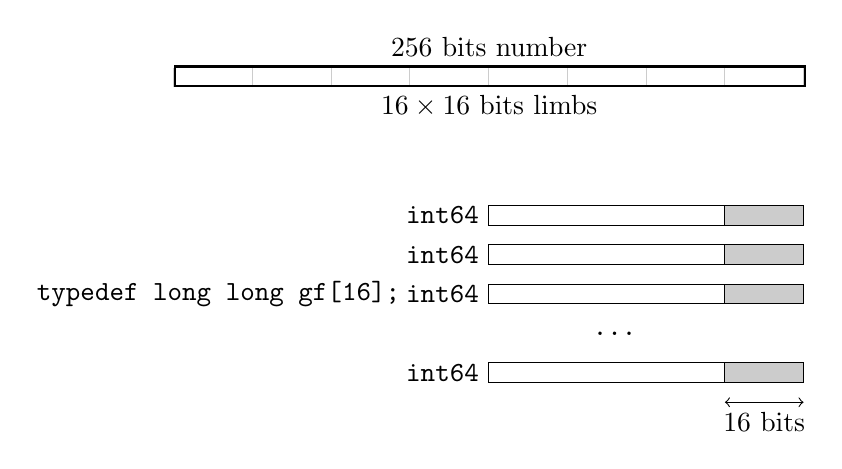
\begin{tikzpicture}[textstyle/.style={black, anchor= south west, align=center}]


  \foreach \x in {0,1,...,8} {
    \draw [black!20] (\x,0) -- (\x,0.25);
  };

  \draw (0,0.25) node[textstyle, minimum width=8cm, minimum height=0.5cm] {$256$ bits number};
  \draw (0,0) node[textstyle, draw=black, thick, minimum width=8cm, minimum height=0.25cm] {};

  \draw (0,-0.5) node[textstyle, minimum width=8cm] {$16 \times 16$ bits limbs};

  \def\yshift{-1.5}
  \def\xshift{4}

  \foreach \y in {0,-0.5,-1,-2} {
    \draw (\xshift+0,\yshift+\y) -- (\xshift+4,\yshift+\y) -- (\xshift+4,\yshift-0.25+\y) -- (\xshift+0,\yshift-0.25+\y) -- cycle;
    \draw [fill=black!20] (\xshift+3,\yshift+\y) -- (\xshift+4,\yshift+\y) -- (\xshift+4,\yshift-0.25+\y) -- (\xshift+3,\yshift-0.25+\y) -- cycle;
    \draw (\xshift,\yshift-0.125+\y) node[anchor= east, align=center] {\texttt{int64}};
  }
  \draw (\xshift+2,\yshift-0.125-1.5) node[anchor= east, align=center] {\texttt{...}};

  \draw (3,\yshift-1.125) node[anchor= east, align=center] {\texttt{typedef long long gf[16];}};

  \def\yshift{-4}
  \draw [<->] (\xshift+3,\yshift) -- (\xshift+4,\yshift);
  \draw (\xshift+3.5,\yshift) node[textstyle, anchor=north] {$16$ bits};



  \end{tikzpicture}

  \end{center}
\end{frame}


%%%%%%%%%%%%%%%%%%%%%%%%%%%%%%%%%
%
%     SLIDE 3
%
%%%%%%%%%%%%%%%%%%%%%%%%%%%%%%%%%
\begin{frame}[fragile]{Basic Operations}
  \begin{center}

\begin{lstlisting}[language=cnacl, caption=Basic Operations, label=cod:languageC31]
#define FOR(i,n) for (i = 0;i < n;++i)
#define sv static void
typedef long long i64;
typedef i64 gf[16];

sv A(gf o,const gf a,const gf b)    # Addition
{
  int i;
  FOR(i,16) o[i]=a[i]+b[i];         # carrying is done separately
}

sv Z(gf o,const gf a,const gf b)    # Zubstraction
{
  int i;
  FOR(i,16) o[i]=a[i]-b[i];         # carrying is done separately
}

sv M(gf o,const gf a,const gf b)    # Multiplication
{
  i64 i,j,t[31];
  FOR(i,31) t[i]=0;
  FOR(i,16) FOR(j,16) t[i+j] = a[i]*b[j];
  FOR(i,15) t[i]+=38*t[i+16];
  FOR(i,16) o[i]=t[i];
  car25519(o);                      # carrying
  car25519(o);                      # carrying
}
\end{lstlisting}

  \end{center}
\end{frame}


%%%%%%%%%%%%%%%%%%%%%%%%%%%%%%%%%
%
%     SLIDE 4
%
%%%%%%%%%%%%%%%%%%%%%%%%%%%%%%%%%
\begin{frame}[fragile]{What needs to be done}
  \begin{center}

  We need to prove:
  \begin{enumerate}
    \item that the operations (A,Z,M) are what they are supposed to be with repect to the number representation
    \item that the operations (A,Z,M) are correct in $GF(2^{255}-19)$.
    \item the absence of possible [over/under]flows.
  \end{enumerate}
  \pause
  \vspace{1cm}
  {\Large Is this enough ?}\\
  \pause
  No! We also need to prove the soundness of {\color[rgb]{0.5,0,0.5}\texttt{car25519}}.
  \end{center}
\end{frame}


%%%%%%%%%%%%%%%%%%%%%%%%%%%%%%%%%
%
%     SLIDE 5
%
%%%%%%%%%%%%%%%%%%%%%%%%%%%%%%%%%
\begin{frame}[fragile]{car25519}
  \begin{center}

\begin{lstlisting}[language=cnacl, caption=car25519, label=cod:languageC51]
sv car25519(gf o)
{
  int i;
  i64 c;
  FOR(i,16) {
    o[i]+=(1LL<<16);
    c=o[i]>>16;
    o[(i+1)*(i<15)]+=c-1+37*(c-1)*(i==15);
    o[i]-=c<<16;
  }
}

# unpacked version:
sv car25519(gf o)
{
  int i;
  i64 c;
  FOR(i,15) {
    o[i]+=(1LL<<16);    # add 2^16
    c=o[i]>>16;         # get the carry (bits > 16)
    o[(i+1)]+=c-1;      # propagate to the next limb
    o[i]-=c<<16;        # remove the carry
  }
  o[15]+=(1LL<<16);     # add 2^16
  c=o[15]>>16;          # get the carry (bits > 16)
  o[0]+=38*(c-1);       # propagate to the first limb
  o[15]-=c<<16;         # remove the carry
}
\end{lstlisting}

  \end{center}
\end{frame}

%%%%%%%%%%%%%%%%%%%%%%%%%%%%%%%%%
%
%     SLIDE 6
%
%%%%%%%%%%%%%%%%%%%%%%%%%%%%%%%%%

\begin{frame}[fragile]{car25519}
  \begin{center}
\begin{lstlisting}[language=cnacl, caption=car25519 in use, label=cod:languageC61]
sv pack25519(u8 *o,const gf n)
{
  int i,j,b;
  gf m,t;
  FOR(i,16) t[i]=n[i];
  car25519(t);
  car25519(t);
  car25519(t);
  ...
\end{lstlisting}

    We need to prove that after $3$ iterations of {\color[rgb]{0.5,0,0.5}\texttt{car25519}},\\
    \Large\alert{all the values in $t$ are below $2^{16}$}.

  \end{center}
\end{frame}

\section{From C to Coq}

%%%%%%%%%%%%%%%%%%%%%%%%%%%%%%%%%
%
%     SLIDE 7
%
%%%%%%%%%%%%%%%%%%%%%%%%%%%%%%%%%

\begin{frame}[fragile]{Proving with VST}
  \begin{center}

  \begin{tikzpicture}[textstyle/.style={black, anchor= south west, align=center}]
      \draw (2.75,0) node[textstyle, anchor=west, draw=yellow, fill=yellow!20, thick, minimum width=5.5cm,minimum height=5cm] {};
      \node[inner sep=0pt] (russell) at (5.5,1.5) {\includegraphics[width=.1\textwidth]{coq_logo.png}};
      \node[inner sep=0pt] (russell) at (5.5,-1.5) {\includegraphics[width=.15\textwidth]{chain.png}};
      \draw (-1,0) node[textstyle, anchor=east, draw=black, thick, minimum width=1cm,minimum height=2cm] {code.c};
      \draw (0.75,-0.5) node[textstyle, anchor=south] {\texttt{clightgen code.c}};
      \draw (4,0) node[textstyle, anchor=east, draw=black, thick, minimum width=1cm,minimum height=2cm] {code.v};
      \draw (8,0) node[textstyle, anchor=east, draw=black, thick, minimum width=1cm,minimum height=2cm] {proofs.v};
      \node[anchor=west,single arrow,draw=red!80!black,fill=red!80!black,minimum width=0.5cm,minimum height=3.25cm] at (-0.75,0) {};
      \node[anchor=west,double arrow,draw=green!60!black,fill=green!60!black,minimum width=0.5cm,minimum height=2.25cm] at (4.25,0) {};
      % \node[anchor=west,double arrow,draw=green!60!black,fill=green!60!black,minimum width=0.5cm,minimum height=2cm] at (3,0) {};
  \end{tikzpicture}

  \end{center}
\end{frame}


%%%%%%%%%%%%%%%%%%%%%%%%%%%%%%%%%
%
%     SLIDE 8
%
%%%%%%%%%%%%%%%%%%%%%%%%%%%%%%%%%

\begin{frame}[fragile]{Specification: ZofList}
  \begin{center}
\begin{lstlisting}[language=Coq, caption=ZofList, label=cod:languageC81]
Variable n: \Z.
Hypothesis Hn: n > 0.

(*
  in C we have gf[16] here we consider a list of integers (list \Z)
  of length 16 in this case.

  ZofList convert a list \Z into it's \Z value
  assume a radix: 2^n
*)
Fixpoint ZofList (a : list \Z) : \Z := match a with
| [] => 0
| h :: q => h + 2^n * ZofList q
end.

Notation "\Z.lst A" := (ZofList A) (at level 65).
\end{lstlisting}

% Lemma ZofList_nil : \Z.lst nil = 0.

% Lemma ZofList_cons_0 : forall a, \Z.lst [a] = a.

% Lemma ZofList_cons :
%   forall a b, \Z.lst a :: b = a + 2^n * \Z.lst b.

% Lemma ZofList_add :
%   forall m a b, \Z.lst m + a :: b = m + \Z.lst a :: b.

% Lemma ZofList_app :
%   forall a b, \Z.lst a ++ b = (\Z.lst a) + 2^(n * \Z.\N (length a)) * \Z.lst b.

  \end{center}
\end{frame}


%%%%%%%%%%%%%%%%%%%%%%%%%%%%%%%%%
%
%     SLIDE 9
%
%%%%%%%%%%%%%%%%%%%%%%%%%%%%%%%%%

\begin{frame}[fragile]{Addition}
  \begin{center}
\begin{lstlisting}[language=Coq, caption=Addition, label=cod:languageC91]
Fixpoint ZsumList (a b : list \Z) : list \Z := match a,b with
| [], q => q
| q,[] => q
| h1::q1,h2::q2 => (Z.add h1 h2) :: ZsumList q1 q2
end.
Notation "A \boxplus B" := (ZsumList A B) (at level 60).

Corollary ZsumList_correct:
  forall (a b: list \Z),
    (\Z.lst a \boxplus b) = (\Z.lst a) + (\Z.lst b).
Qed.

Lemma ZsumList_bound_len:
  forall (m1 n1 m2 n2: \Z) (a b: list \Z),
    length a = length b ->
    Forall (fun x => m1 < x < n1) a ->
    Forall (fun x => m2 < x < n2) b ->
      Forall (fun x => m1 + m2 < x < n1 + n2) (a \boxplus b).
Qed.
\end{lstlisting}

  \end{center}
\end{frame}

%%%%%%%%%%%%%%%%%%%%%%%%%%%%%%%%%
%
%     SLIDE 10
%
%%%%%%%%%%%%%%%%%%%%%%%%%%%%%%%%%

\begin{frame}[fragile]{Multiplication - specification}
  \begin{center}
\begin{lstlisting}[language=cnacl, caption=M, label=cod:languageC101]
sv M(gf o,const gf a,const gf b)    # Multiplication
{
  FOR(i,16) FOR(j,16) t[i+j] = a[i]*b[j];   # mult_1
  FOR(i,15) t[i]+=38*t[i+16];               # mult_2
  FOR(i,16) o[i]=t[i];                      # mult_3
 }
\end{lstlisting}

\begin{lstlisting}[language=Coq, caption=Multiplication, label=cod:languageC102]
Fixpoint ZscalarMult (a: \Z) (b: list \Z) : list \Z := match b with
| [] => []
| h :: q => a * h :: ZscalarMult a q
end.
Notation "A \circ B" := (ZscalarMult A B) (at level 60).

Fixpoint mult_1 (a b:list \Z) : list \Z := match a, b with
| [],_ => []
| _,[] => []
| ha :: qa, hb :: qb => ha * hb :: (ha \circ qb) \boxplus (mult_1 qa (hb::qb))
end.

Definition mult_2 (a:list \Z) : list \Z := a  \boxplus (38 \circ (tail 16 a)).
(* where "tail n a" drop the n first elements of a *)

Definition mult_3 (a:list \Z) : list \Z := slice 16 a.
(* where "slice n a" keep the n first elements of a *)

Definition M (a b:list \Z) : list \Z := mult_3 (mult_2 (mult_1 a b)).
\end{lstlisting}

  \end{center}
\end{frame}

%%%%%%%%%%%%%%%%%%%%%%%%%%%%%%%%%
%
%     SLIDE 11
%
%%%%%%%%%%%%%%%%%%%%%%%%%%%%%%%%%

\begin{frame}[fragile]{Multiplication - correctness}
  \begin{center}
\begin{lstlisting}[language=Coq, caption=Multiplication | proof of correctness, label=cod:languageC111]
Notation "A :\GF" := (A mod (2^255 - 19)) (at level 40).

Corollary mult1_correct :
  forall (a b: list \Z),
    \Z.lst mult_1 a b =  (\Z.lst a) * (\Z.lst b).
Qed.

Lemma mult_2_correct :
  forall (l: list \Z),
    (\Z.lst mult_2 l) = (\Z.lst l) + 38 * \Z.lst tail 16 l.
Qed.

Lemma reduce_slice_GF:
  forall (l: list \Z),
    \Z.\N length l < 32 ->
      (\Z.lst mult_3 (mult_2 l)) :\GF = (\Z.lst l) :\GF.
Qed.

Corollary mult_GF:
  forall (a b: list \Z),
    \Z.\N length a = 16 ->
    \Z.\N length b = 16 ->
      (\Z.lst M a b) :\GF = (\Z.lst a) * (\Z.lst b) :\GF.
Qed.
\end{lstlisting}

  \end{center}
\end{frame}


%%%%%%%%%%%%%%%%%%%%%%%%%%%%%%%%%
%
%     SLIDE 12
%
%%%%%%%%%%%%%%%%%%%%%%%%%%%%%%%%%

% \begin{frame}[fragile]{Multiplication - base lemma}
%   \begin{center}
% \begin{lstlisting}[language=Coq, caption=Base lemma for the multiplication, label=cod:languageC121]
% Definition min_prod (min1 max1 min2 max2: \Z) : \Z :=
%   Zmin (Zmin (min1*min2) (max1*max2)) (Zmin (max1*min2) (min1*max2)).

% Definition max_prod (min1 max1 min2 max2: \Z) : \Z :=
%   Zmax (Zmax (min1*min2) (max1*max2)) (Zmax (max1*min2) (min1*max2)).

% Lemma Mult_interval_correct_min_max_lt :
%   forall a b c d x y : \Z,
%     a < x < b ->
%     c < y < d ->
%     min_prod a b c d < x * y < max_prod a b c d.
% Qed.
% \end{lstlisting}

%   \end{center}
% \end{frame}

%%%%%%%%%%%%%%%%%%%%%%%%%%%%%%%%%
%
%     SLIDE 13
%
%%%%%%%%%%%%%%%%%%%%%%%%%%%%%%%%%

\begin{frame}[fragile]{Multiplication - bounds}
  \begin{center}
\begin{lstlisting}[language=Coq, caption=Multiplication | Proofs of bounds, label=cod:languageC131]
Lemma ZscalarMult_bound_const:
  forall (m2 n2 a: \Z) (b: list \Z),
    0 < a ->
    Forall (fun x => m2 < x < n2) b ->
    Forall (fun x => a * m2 < x < a * n2) (a \circ b).
Qed.

Lemma mult_1_bound:
  forall (m1 n1 m2 n2 m3 n3: \Z) (a b: list \Z),
    (fun x => m1 < x < n1) 0 ->
    (fun x => m2 < x < n2) 0 ->
    Forall (fun x => m1 < x < n1) a ->
    Forall (fun x => m2 < x < n2) b ->
    m3 = Zmin (Zlength a) (Zlength b) * min_prod m1 n1 m2 n2 ->
    n3 = Zmin (Zlength a) (Zlength b) * max_prod m1 n1 m2 n2 ->
      Forall (fun x => m3 < x < n3) (mult_1 a b).
Admitted.

Lemma mult_2_bound:
  forall (m1 n1: \Z) (a: list \Z),
    (fun x => m1 < x < n1) 0 ->
    Forall (fun x => m1 < x < n1) a ->
      Forall (fun x => m1 + 38 * m1 < x < n1 + 38 * n1) (mult_2 a).
Qed.

Lemma mult_3_bound:
  forall (m1 n1: \Z) (a: list \Z),
    Forall (fun x => m1 < x < n1) a ->
      Forall (fun x => m1 < x < n1) (mult_3 a).
Qed.
\end{lstlisting}

  \end{center}
\end{frame}


%%%%%%%%%%%%%%%%%%%%%%%%%%%%%%%%%
%
%     SLIDE 14
%
%%%%%%%%%%%%%%%%%%%%%%%%%%%%%%%%%

\begin{frame}[fragile]{Multiplication - bounds}
  \begin{center}
\begin{lstlisting}[language=Coq, caption=M | Proofs of bounds, label=cod:languageC141]
Lemma mult_bound:
  forall (m1 n1 m2 n2 m3 n3: Z) (a b: list Z),
    (fun x => m1 < x < n1) 0 ->
    (fun x => m2 < x < n2) 0 ->
    Forall (fun x => m1 < x < n1) a ->
    Forall (fun x => m2 < x < n2) b ->
    m3 = 39 * Z.min (Zlength a) (Zlength b) * min_prod m1 n1 m2 n2 ->
    n3 = 39 * Z.min (Zlength a) (Zlength b) * max_prod m1 n1 m2 n2 ->
      Forall (fun x => m3 < x < n3) (M a b).
Admitted.
\end{lstlisting}

  \end{center}
\end{frame}

\begin{frame}[fragile]{Multiplication - bounds}
  What can we deduce from this ?
  \begin{center}
  \begin{align*}
    39 \times 16 \times (2^x)^2 &< 64 \times 16 \times (2^x)^2\\
    64 \times 16 \times (2^x)^2 &< 2^{62}\\
    2^6 \times 2^4 \times (2^x)^2 &< 2^{62}\\
    x &< 26
  \end{align*}
  Thus we will avoid any over/underflows if the inputs are within the $]-2^{26},2^{26}[$ ranges:
 \begin{lstlisting}[language=Coq, caption=M | Proofs of bounds, label=cod:languageC141]
Lemma mult_bound_strong:
  forall (a b: list Z),
    (length a = 16)%\N ->
    (length b = 16)%\N ->
    Forall (fun x => -2^26 < x < 2^26) a ->
    Forall (fun x => -2^26 < x < 2^26) b ->
      Forall (fun x => -2^62 < x < 2^62) (M a b).
Admitted.
\end{lstlisting}

  \end{center}
\end{frame}

\section{car25519}

%%%%%%%%%%%%%%%%%%%%%%%%%%%%%%%%%
%
%     SLIDE 15
%
%%%%%%%%%%%%%%%%%%%%%%%%%%%%%%%%%

\begin{frame}[fragile]{car25519 - specification}
  \begin{center}

\begin{lstlisting}[language=cnacl, caption=car25519 | propagation, label=cod:languageC151]
  FOR(i,15) {
    o[i]+=(1LL<<16);    # add 2^16
    c=o[i]>>16;         # get the carry (bits > 16)
    o[(i+1)]+=c-1;      # propagate to the next limb
    o[i]-=c<<16;        # remove the carry
  }
\end{lstlisting}

\begin{lstlisting}[language=Coq, caption=car25519 | Proofs of correctness, label=cod:languageC152]
(*
  getCarry n m      is equivalent to    m >> n
  getResidute n m   is equivalent to    m mod 2^n
*)

Fixpoint Carrying_n (p:\N) (a:\Z) (l:list \Z) : list \Z := match p,a,l with
| _,  0,[]     => []
| _,  a,[]     => [a]
| 0%\N,  a,h::q => (a + h) :: q
| S p,a,h :: q => getResidute n (a + h) :: Carrying_n p (getCarry n (a + h)) q
end.

Corollary CarrynPreserve:
  forall (m: \N) (l: list \Z),
    \Z.lst l = \Z.lst Carrying_n m 0 l.
Qed.
\end{lstlisting}

Remark: the add $2^{16}$ step has been ignored.
  \end{center}
\end{frame}


%%%%%%%%%%%%%%%%%%%%%%%%%%%%%%%%%
%
%     SLIDE 16
%
%%%%%%%%%%%%%%%%%%%%%%%%%%%%%%%%%

\begin{frame}[fragile]{car25519 - specification}
  \begin{center}

\begin{lstlisting}[language=cnacl, caption=car25519 | back, label=cod:languageC161]
  o[15]+=(1LL<<16);     # add 2^16
  c=o[15]>>16;          # get the carry (bits > 16)
  o[0]+=38*(c-1);       # propagate to the first limb
  o[15]-=c<<16;         # remove the carry
\end{lstlisting}

\begin{lstlisting}[language=Coq, caption=car25519 | Proofs of correctness, label=cod:languageC162]
Definition backCarry (l:list Z) : (list Z) :=
  match l with
  | [] => []
  | h :: q => let v := nth 15 l 0 in
              (h + 38 * getCarry 16 v) :: slice 14 q ++ [getResidute 16 v]
  end.

Lemma backCarry_25519:
  forall (l:list \Z),
    (length l <= 16)%\N ->
      (\Z.lst l) :\GF  = ((\Z.lst backCarry l) :\GF).
Qed.
\end{lstlisting}

  \end{center}
\end{frame}



%%%%%%%%%%%%%%%%%%%%%%%%%%%%%%%%%
%
%     SLIDE 17
%
%%%%%%%%%%%%%%%%%%%%%%%%%%%%%%%%%

\begin{frame}[fragile]{car25519 - correctness \& bounds}
  \begin{center}
\begin{lstlisting}[language=Coq, caption=car25519 | Proofs of correctness, label=cod:languageC171]
Definition car25519 (l:list \Z) : list \Z := backCarry (Carrying_n 16 15 0 l).

Lemma car25519_correct:
  forall (l: list \Z),
    (length l = 16)%\N ->
      (\Z.lst l) :\GF  = (\Z.lst car25519 l) :\GF.
Qed.

Lemma car25519_bound :
  forall (i: \N) (l: list \Z),
    (length l = 16)%\N ->
    (i <> 0)%\N ->
      nth i (car25519 l) 0 < 2 ^ 16.
\end{lstlisting}
  \end{center}
\end{frame}



%%%%%%%%%%%%%%%%%%%%%%%%%%%%%%%%%
%
%     SLIDE 18
%
%%%%%%%%%%%%%%%%%%%%%%%%%%%%%%%%%

\begin{frame}[fragile]{car25519 - bounds}
  \begin{center}
\begin{lstlisting}[language=Coq, caption=car25519, label=cod:languageC181]
Lemma t2256is38 : (2^256 :\GF) = (38 :\GF).
Proof. compute. reflexivity. Qed.

Definition Zcar25519 (n: \Z) : \Z  :=  38 * getCarry 256 n +  getResidute 256 n.

Lemma Zcar25519_correct:
  forall (n: \Z), n :\GF = (Zcar25519 n) :\GF.
Qed.

Lemma Zcar25519_eq_car25519:
  forall (l : list \Z),
  (length l = 16)%\N ->
    Zcar25519 (\Z.lst l) = \Z.lst (car25519 l).
Qed.
\end{lstlisting}

  \end{center}
\end{frame}


%%%%%%%%%%%%%%%%%%%%%%%%%%%%%%%%%
%
%     SLIDE 19
%
%%%%%%%%%%%%%%%%%%%%%%%%%%%%%%%%%

\begin{frame}[fragile]{car25519 - bounds}
  \begin{center}
\begin{lstlisting}[language=Coq, caption=car25519, label=cod:languageC191]
Lemma ZCarry25519_min:
  forall (x: \Z),
    0 < x ->
      0 < Zcar25519 x.
Qed.

Lemma ZCarry25519_sup_bounds:
  forall (x: \Z),
    x < 2 ^ 302 ->
    0 < x ->
      Zcar25519 x < 2 ^ 257.
Qed.

Lemma Zcarry25519_fixpoint :
  forall (x: \Z),
  0 < x < 2 ^ 256 ->
    Zcar25519 x = x.
Qed.

Theorem doubleCar:
  forall (x y: \Z),
    0 <= x < 2 ^ 302 ->
    y = Zcar25519 x ->
      Zcar25519 y < 2 ^ 256.
Qed.
\end{lstlisting}

  \end{center}
\end{frame}

\begin{frame}[standout]
  \Huge What is left ?
\end{frame}

\begin{frame}[fragile]{Work In Progress}
    Curent and future work:
    \begin{itemize}
      \item finish the proofs on the bounds for the Multiplication.
      \item redo all the proofs on the carrying including the addition of $2^{16}$.
      \item Prove that the model matches the semantic (\texttt{code.v}) using VST (\#Princeton).
      \item Prove that the steps does not yeld to an over/underflow.
    \end{itemize}
\end{frame}


% Fixpoint ZsubList (a b : list Z) : list Z := match a,b with
% | [], q => ZminusList q
% | q,[] => q
% | h1::q1,h2::q2 => (Z.sub h1 h2) :: ZsubList q1 q2
% end.

% Notation "A \ominus B" := (ZsubList A B) (at level 60).


%%%%%%%%%%%%%%%%%%%%%%%%%%%%%%%%%
%
%     SLIDE 14
%
%%%%%%%%%%%%%%%%%%%%%%%%%%%%%%%%%
\begin{frame}[standout]
	\Huge Thank you.
\end{frame}

\end{document}